\chapter{Path Planning}
\label{chapter:path_planning}

\textbf{Author: Fabian Kleinrad} 

A crucial part of autonomy in robotics are the means for planning ahead movements in a cooperative manner with the environment. Methods to accomplish this, are generally referred to as path planning algorithms. This chapter is going to focus on exploring different kinds of approaches to path planning and evaluate which approach is most fitting to be used in a real-time, high-dimensional use case present in the autumn project.


\section{Types of Path Planning}

The problem of finding an optimal path between two points is an old one.
The first proposed solution was the Dijkstra's algorithm. However, with steadily evolving computer science the challenges to be mastered by such algorithms got harder and harder. That's the reason why over the last years the simple principle of the Dijkstra algorithm has branched out specializing and excelling in certain real-world applications.
\footcite{Pan2020}

\subsection{Sampling-based Algoritms}

In motion planning, sampling-based algorithms can be differentiated to other kinds of approaches, by the way, they explore their environment. sampling-based algorithms such as the probabilistic road map algorithm or the rapidly exploring random tree use a random point in their reference space and expand in that direction. This random point is considered a sample.

\subsection{Multiple-Query and Single-Query}

The term multiple-query refers, in connection with path planning Algorithms, to the feasibility of deriving a variety of different paths, without the need of rerunning the algorithm. In contrast, single-query algorithms are only able to compute one path at a time.\newline
Use cases for Multiple-Query Algorithms would be unchanging environments. The reason for that, by generating an extensive grid of connections to be able to calculate a multitude of different start/goal combinations  more computational time is needed.\newline
Single-Query approaches focus on performance instead of reuse-ability, which makes them ideal for dynamic domains. 
\footcite{Bekris2003}
\footcite{stackexchangeMultiSingleQuery2019}

\section{PRM}

Probabilistic RoadMap is a path planning algorithm tailored to multi-query applications. It is considered one of the most influential sampling-based path planning algorithms. 

The algorithm can be broken down into two phases. The first phase, which is referred to as the pre-processing phase, starts with an empty graph. At first, it samples n random points and adds them to a set of vertices if they are located in space free from obstacles. After constructing a set of n vertices, it attempts connections between a random vertex and its neighboring nodes in a predefined radius. This connecting of to vertices is realized with a simple straight-line connection. All collision-free connections between vertices and their respective neighbors are added to a set of edges. The result of this pre-processing phase is a roadmap, with the number of sampled points determining the quality of to be calculated paths. 
\footcite{Karaman2011}

Upon finishing the initial construction phase of a roadmap, like the one depicted in figure 8.1, start/goal combinations can be processed. 
The actual path finding in the generated graph is handled by other non-sampling-based path finding methods such as A*.\newline
With the PRM focusing on a multi-query approach it is possible to calculate an arbitrary number of different paths without the need to construct a new graph.

\begin{figure}[h]
	\centering
	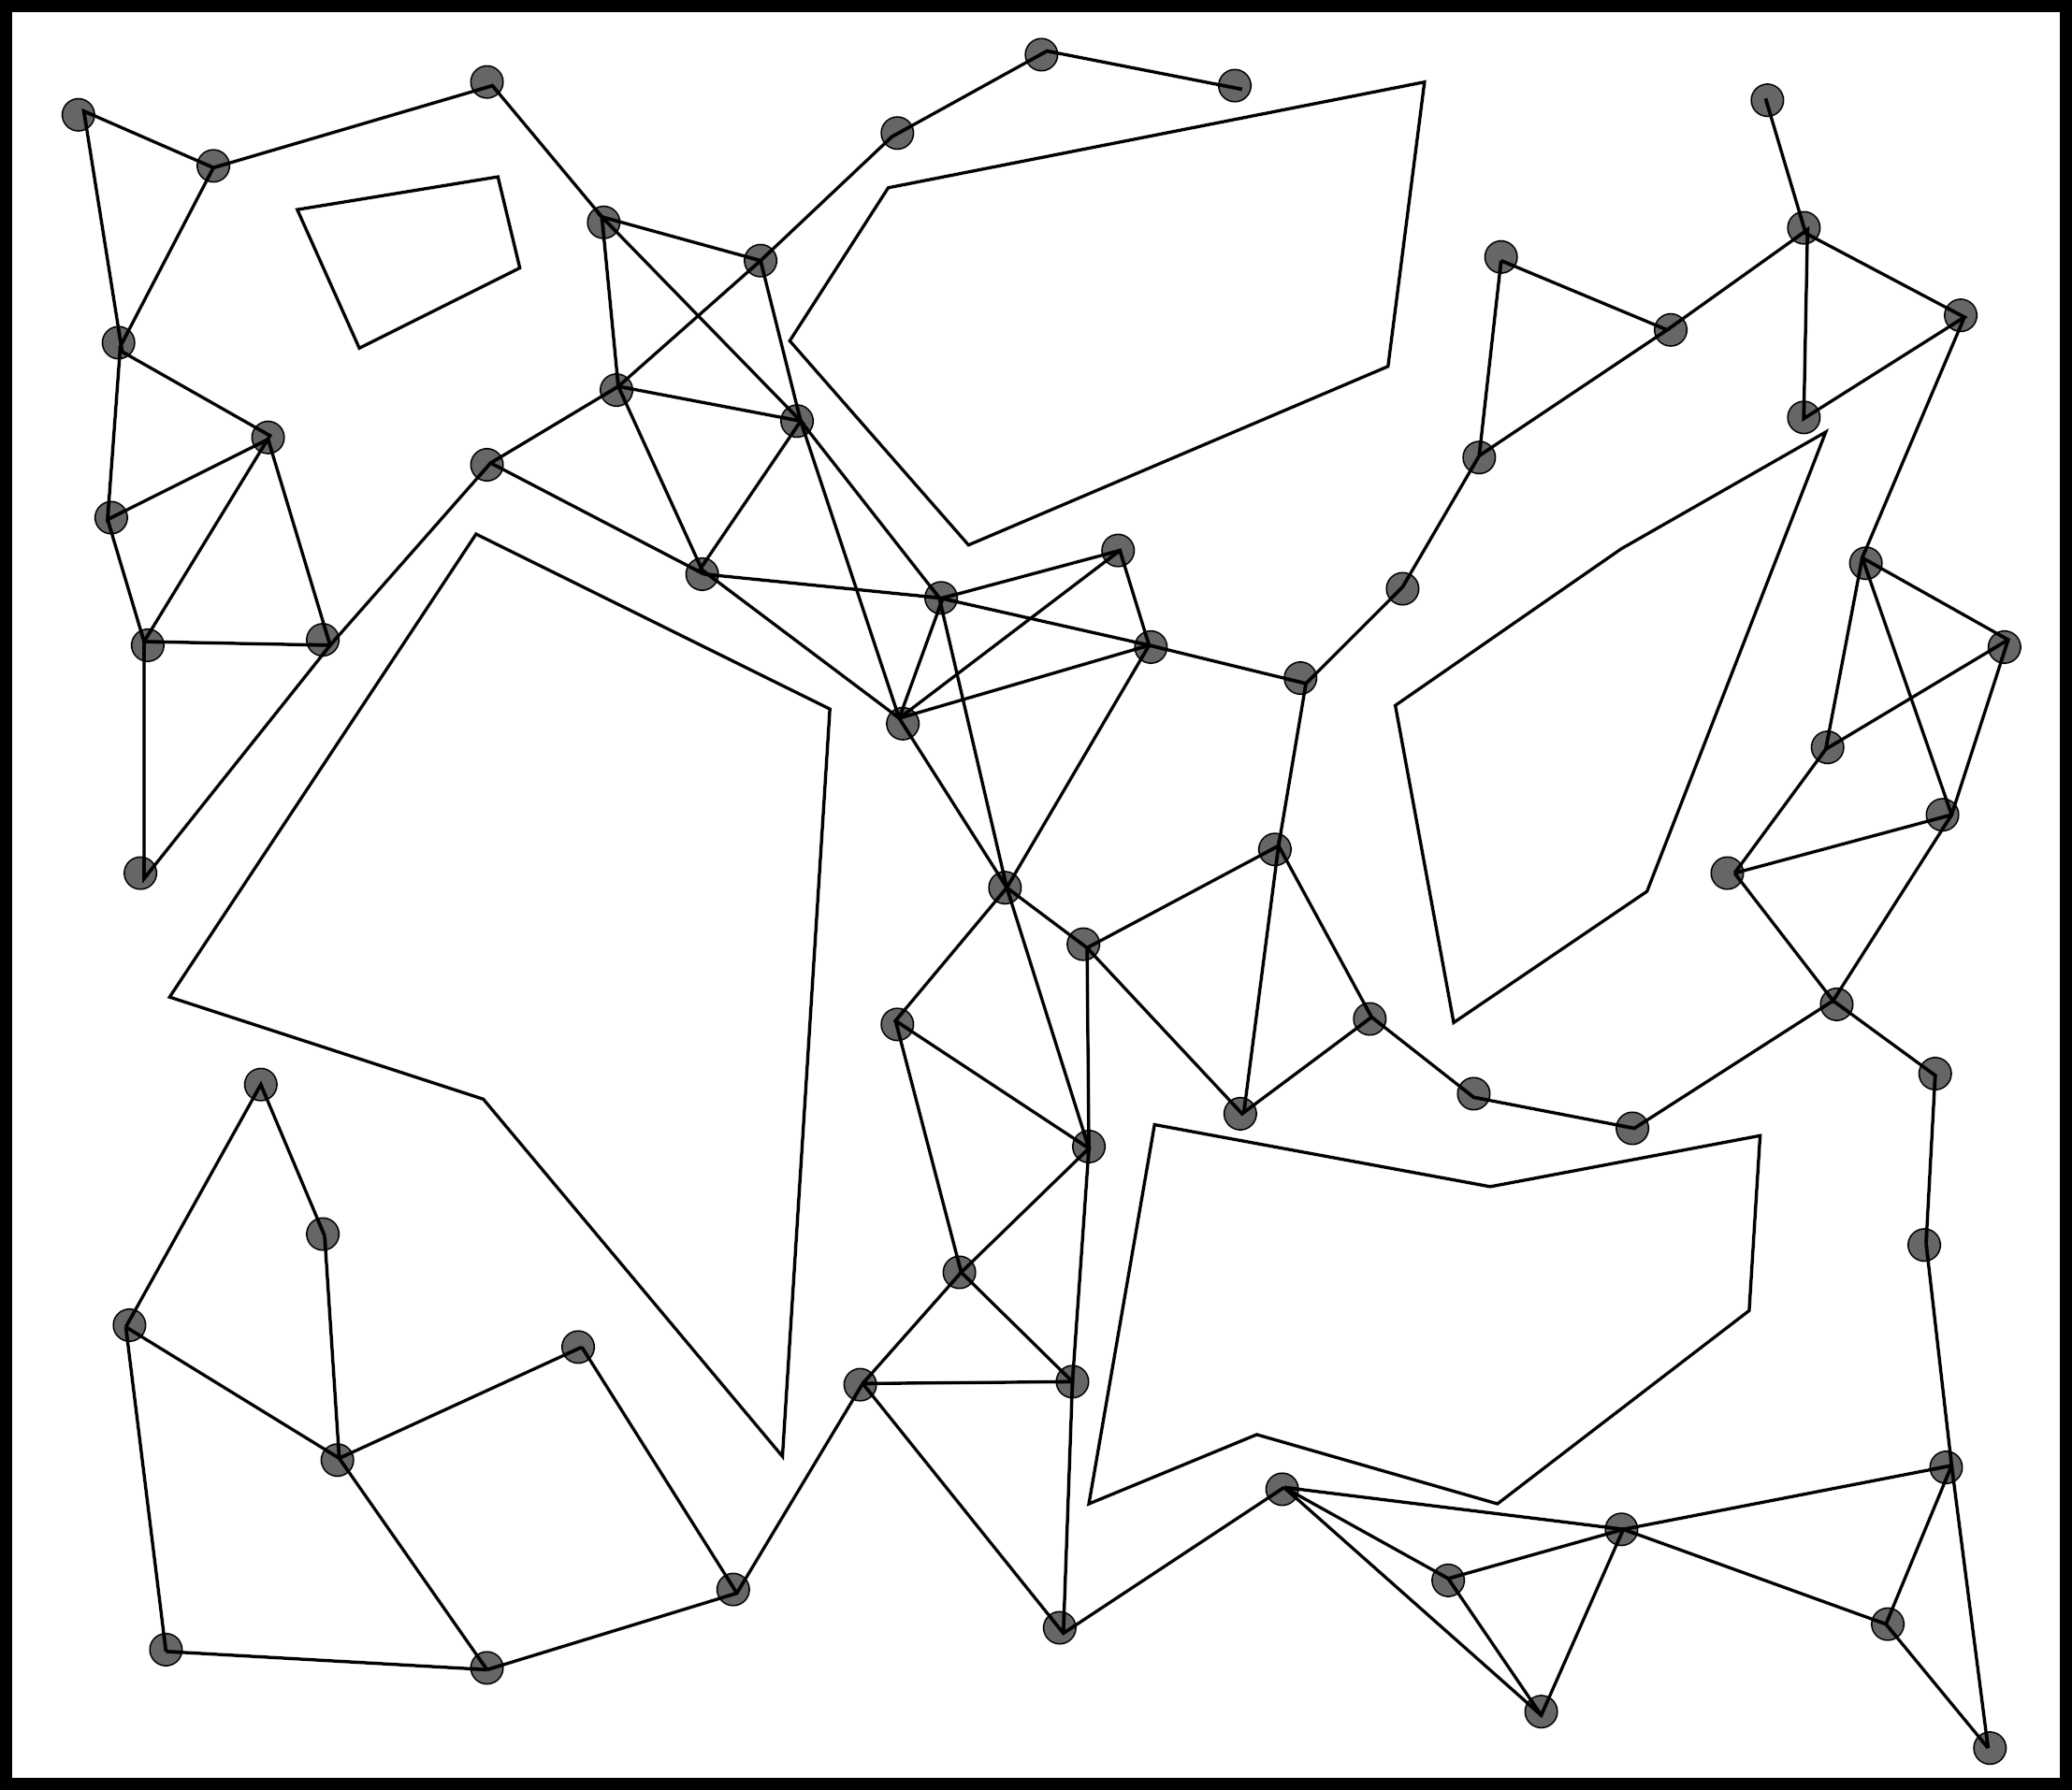
\includegraphics[width=0.7\linewidth]{img/PRMRoadmap}
	\caption{Example of a roadmap in two dimensional space constructed by the PRM algorithm.}
	\label{fig:path_planning_prm}
\end{figure}

\section{RRT Algorithm}

Rapidly exploring random tree is a path planning algorithm, that can be categorized as sampling-based and single-query. In the field of sampling-based path-finding algorithms is it considered together with the PRM the most influential. RRT works by constructing a tree of possible trajectories. Therefore it is first required to define an initial vertex, much like a root. After each following iteration, a random sample is taken from the space that is considered free from obstacles. After generating a random vertex, the nearest neighboring point in the tree is searched for. The closest node is then used as a pivot point and a new vertex is constructed a predefined distance away from the nearest node in the direction of the random sample. Thereafter it is attempted to connect the new vertex with the nearest. If this straight-line connection can exit without colliding with obstacles it is added to the set of edges. This procedure is depicted in figure 8.2. The algorithm ends when a new node is within the predefined distance away from the goal point. 
\footcite{Karaman2011}

The name rapidly exploring random tree stems from the tree-like structure constructed, like the one you can see in figure 8.2 when exploring spaces This approach to path planning makes it possible to explore rapidly changing environments efficiently.


\begin{figure}[h]
	\centering
	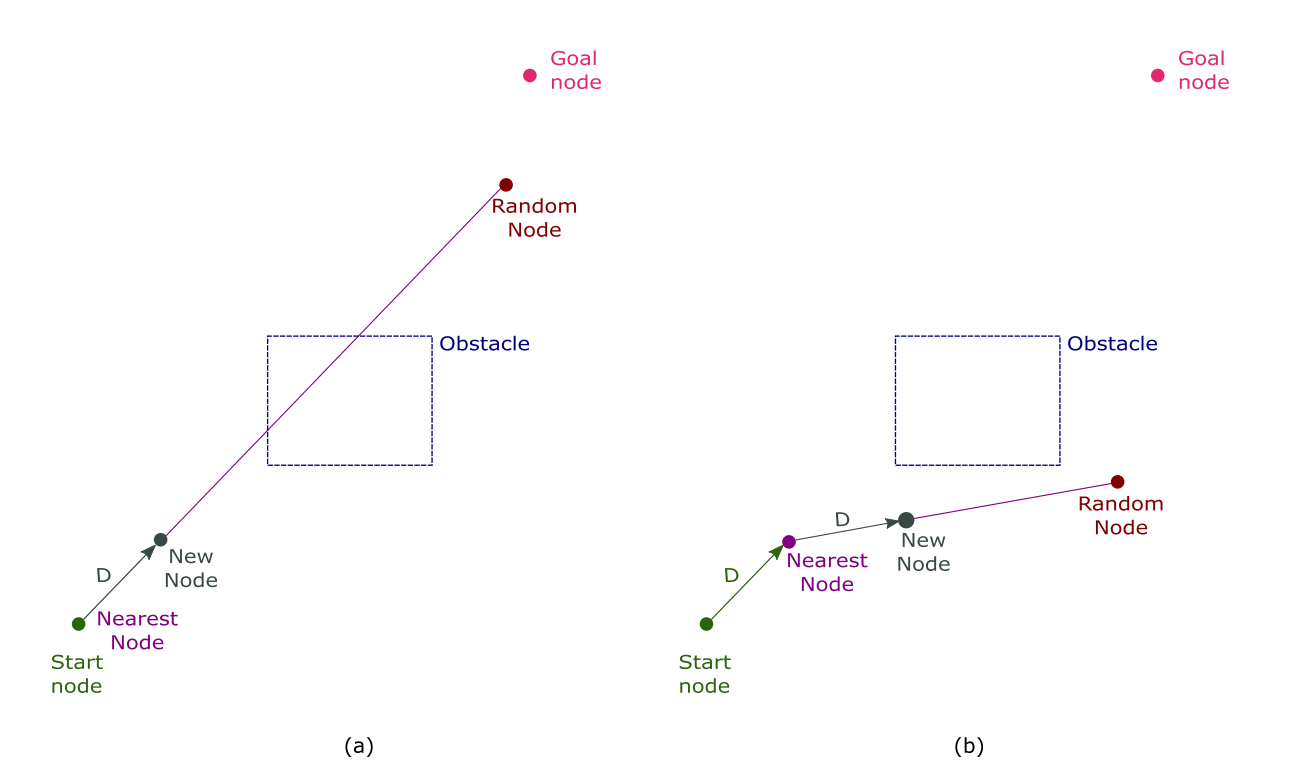
\includegraphics[width=0.9\linewidth]{img/rrtIteration}
	\caption{Visualization of the first two iterations (a), (b) when an rrt algorithm is exploring a simple 2d space with an obstacle present. D referring to the predefined distance between vertices.\footcite{Zammit2018}}
	\label{fig:path_planning_rrt}
\end{figure}

\section{A* Algorithm}

The A* algorithm is a simplistic and reliable method compared to other path-planning techniques. Therefore it is nowadays prevalently used in a variety of different applications.\footcite{Zammit2018}\newline
It combines heuristic properties with formal virtues of Dijkstra's algorithm. Whereas a purely heuristic approach would not guarantee that a path can be found even if a possible solution existed, the A* guarantees that the shortest path is found.\footcite{Sathyaraj2008}
A* works by trying all possible combinations like the Dijkstra algorithm in a grid or graph-based environment. With A* being based on the Dijkstra algorithm it favors nodes that are closer to the current position. Additionally, it follows heuristic principles by putting a higher priority on nodes closer to the goal. An example of what an A* search algorithm looks like in a grid-based environment is depicted in figure. 8.3.\footcite{standfordAStarComparison1997}\newline
With these properties, it can be considered an informed Dijkstra search.
  
\begin{figure}[h]
	\centering
	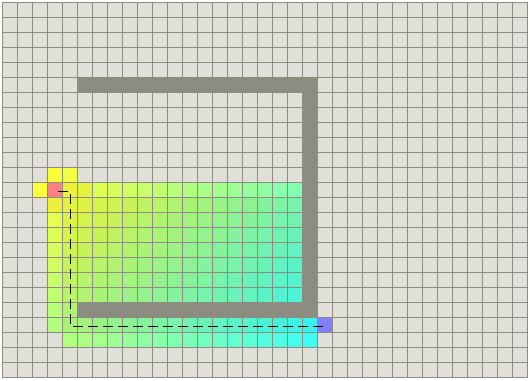
\includegraphics[width=0.7\linewidth]{img/AStarExample}
	\caption{A* path finding around a concave obstacle in a grid-based environment.\footcite{standfordAStarComparison1997}}
	\label{fig:path_planning_Astar}
\end{figure}

\section{Evaluation}

This section is going to cover the reasons behind the selection of the path-planning algorithm used in autumn. Therefor we are going to theoretically evaluate the performance of each algorithm in relation to the environment provided by the project. Additionally, we are going to focus on properties essential for accomplishing the goal set in the autumn project.

\subsection{Autumn Use-case}

There are several criteria to be fulfilled, in order to be considered a working solution for the challenge of path planning faced by Autumn.
As a means to use one of the aforementioned algorithms, they have to be suitable for a real-time, 3-dimensional application, like the one present in the project.
When working with UAVs it is critical that an optimal path is calculated reliable and in the shortest amount of time possible. 

\subsection{Comparison}

In the following comparison, we are going to look at the performance of the three different algorithms already mentioned in this chapter. Knowing that the PRM algorithm doesn't find a path on its own, it is implied from here on out that the PRM works in combination with the A* algorithm and the A* on its own is only applied with grid-based environments.  

\subsubsection{Computational time requirement}

An important requirement to be fulfilled by the path planning algorithm of the Autumn project is to require as little computational time as possible. Taking a look at the PRM algorithm, with its principle of reusing the generated graph, as a road-map, resulting in a short runtime of the algorithm, when looking at the computation of multiple paths. The best-case scenario for the PRM in this configuration would be, an A* algorithm running in a graph-based environment, with the PRM only having to do generate the graph and improve it progressively. A problem that arises is that this best-case scenario is impossible to happen in the Autumn project. Starting uneducated about the environment, like in Autumn, is the worst case for the PRM. At first, the PRM algorithm would generate a road-map in an environment where most of the obstacles are still unknown. Thereafter when the drone gets its first path to its destination it detects obstacles and expands the known space for the algorithm. With the environment changing as much as in Autumn it would be far too expensive to rewire the existing road-map around new obstacles. A* is the best-case scenario in a graph-based environment for the PRM, but what about running the A* standalone now in a grid-based environment. Grid-based environments tend to be very resource-intensive, with full coverage of the entire space. To preclude the possibility of large portions of the search being dissipated, the A* is biased towards the goal. When comparing the A* to the PRM in terms of computational speed in Autumn, A* would be superior, because of the substantial amount of time the PRM takes to generate a road-map only to discard it a few iterations later. That being said, the A* still needs to cover a vast grid, depending on the granularity of the grid. Know knowing that both the A* and PRM algorithms aren't the most efficient in the matter of short runtime, let's cover the RRT algorithm. With RRT following a graph-based and sampling-based approach like the PRM, it covers the space to be explored within a short time frame. The RRT, in contrast to the PRM, doesn't take time to construct the graph and then start to find a path. RRT searches for a path while constructing the tree-like structure. This results in the fastest computational time of all other mentioned algorithms when looking at one-time path planning. With the reference space of the algorithm in Autumn being drastically and continuously changing, it resembles a one-time use path perfectly fitted to be determined by a single-query path planning algorithm like the RRT.

\subsubsection{Scalability for high-dimensional spaces}

Thus far the application of proposed algorithms happened in a two-dimensional environment. When working with UAVs, there is the added challenge of a third dimension to be covered, in contrast to using ground-based vehicles. This added dimension imposes new challenges that the whole system has to handle, with the means to plan a path being one of the most affected.
Additional time complexity being the most crucial change when working in a higher dimension, it is essential to be as efficient as possible. The last point covered the time required for each algorithm. With most path-planning algorithms having a time complexity of \(O\left(b^d\right)\)\footcite{stackexchangeAstarTimeComplexity2019}. With A* being one of the most time-intensive.
In this equation, the variable $b$ is the branching factor and describes the number of descendants of a parent node. $d$ refers to the depth of the goal node. The worst-case scenario would be \(O\left(|V|\right)\), meaning that every vertex of the reference space has to be checked. Looking at the problem of three dimensions where the added dimension increases the number of vertices exponentially. A* being a simple approach with brute force characteristics isn't suitable for application in high dimensional spaces. 

Comparing the RRT to the A* highlights the benefits of a sampling-based approach. While the A* looks at direct neighbours to continue the search, RRT has a step range as a predefined constant. Therefore the RRT explores with a faster pace due to a rougher coverage of the space. This means in relation to higher dimensional spaces it converges more efficiently than the A*.

\subsection{Conclusion}

By evaluating the potential algorithms to be used in the autumn project, the RRT came out on top. With each algorithm providing unique features best fitted for the use-case they are designed for, the problems the RRT algorithm tries to solve are the same encountered in autumn. Properties like space complexity and path quality were neglected in this comparison, due to the low importance of the project. By shifting the computation away from the drone the importance of minimum time far outweighs the required space. Furthermore, the need for an optimal path isn't required on account of the goal being to cover the whole space eventually. That being said a big drawback of the base RRT algorithm is the incapability to provide the possibility to improve on an existing path by rewiring the graph. For that, we are going to take a look at a variant of RRT the RRT* that solves this exact problem.


\section{RRT* Algorithm}

This section is going to cover the improved version of the RRT algorithm, mentioned above. The RRT* algorithm is being used in the Autumn project as the path planning algorithm. The rationale for this decision is covered in the evaluation section. 

\subsection{Concept behind RRT*}

A problem that arises when using the RRT algorithm is that finding an optimal path is impossible due to the lack of rewiring options. Therefore the RRT* algorithm was invented. 
The improved algorithm works differently when connecting a newly sampled node into the existing tree structure, which in the RRT is done by connecting the new node to its nearest neighbour. In the case of the RRT*, it calculates the cost of other possible connections stemming from the root node. Hereby a set of nodes closest to the newly sampled vertex are used as possible connection candidates. By rewiring the tree after each new node is sampled it makes it possible for a near-optimal path to be found.

\subsection{Algorithm}

The RRT* works at first the same as the RRT algorithm, it first defines a set of vertices, $V$ with the start node and an empty set of Edges, $E$. In contrast to the RRT algorithm is the runtime of the RRT* algorithm is not dependent on how fast the goal node is reached, but instead on the degree of optimization for the calculated path.
Line four to six in Algorithm 1, are the same as the base algorithm. Hereby is a random node sampled, the nearest node in relation to the random node is calculated and a new node generated. After checking if a straight-line connection is possible between $x_{nearest}$ and $x_{new}$, a set of neighbouring vertices, $X_{near}$ is initialized.
$X_{near}$ consist of nodes in the tree with a distance $D$, in relation to $x_{new}$. Thereafter $x_{new}$ gets added to the $V$. In lines 9 to 13, the cost of paths connecting the nodes of $X_{near}$ with $x_{new}$ get calculated and an edge between the node with the cheapest path, $x_{min}$ and $x_{new}$ gets added to $E$. The final stage of the RRT* is to rewire all neighbouring nodes in $X_{near}$, if the path connecting to $x_{new}$ is cheaper than the original path to the root vertex. 

\begin{algorithm}[H]
	\caption{RRT* 2011\footcite{Karaman2011}}
	\SetKwFunction{FObstacleFree}{ObstacleFree}
	\SetKwFunction{FSampleFree}{SampleFree}
	\SetKwFunction{FNearest}{Nearest}
	\SetKwFunction{FNear}{Near}
	\SetKwFunction{FCost}{Cost}
	\SetKwFunction{FCollisionFree}{CollisionFree}
	\SetKwFunction{FSteer}{Steer}
	\SetKwFunction{FLine}{Line}
	$V \gets \{x_{init}\}$\;
	$E \gets 0$\;
	\For{$i \gets 1$ \textbf{to} $n$} {
		$x_{rand} \gets \FSampleFree()$\;
		$x_{nearest} \gets \FNearest(G = (V, E), x_{rand})$\;
		$x_{new} \gets \FSteer(x_{nearest}, x_{rand}, D)$\;
		\If{\FObstacleFree($x_{nearest}$, $x_{new}$)}{
			$X_{near} \gets \FNear(G = (V, E), x_{new}, D)$\;
			$V \gets V \cup \{x_{new}\}$\;
			$x_{min} \gets x_{nearest}$\;
			$c_{min} \gets \FCost(x_{nearest}) + c(\FLine(x_{nearest}, x_{new}))$\;
			\ForEach{$x_{near} \in X_{near}$} {
				\If{\FCollisionFree($x_{near}$, $x_{new}$) $\land$ \FCost($x_{near}$) + $c(\FLine(x_{near}, x_{new})) < c_{min}$}{
					$x_{min} \gets x_{near}$\;
					$c_{min} \gets \FCost(x_{near}) + c(\FLine(x_{near}, x_{new}))$\;
				}
			}
			$E \gets E \cup \{(x_{min}, x_{new})\}$\;
			\ForEach{$x_{near} \in X_{near}$} {
				\If{\FCollisionFree($x_{near}$, $x_{new}$) $\land$ \FCost($x_{new}$) + $c(\FLine(x_{near}, x_{new})) < c_{near}$}{
					$x_{parent} \gets Parent(x_{near})$\;
				}
				$E \gets (E \backslash \{(x_{parent}, x_{near})\} \cup \{(x_{new}, x_{near})\})$\;
			}
		}
	}
	\Return G = (V, E);
\end{algorithm}

\section{RRT* Variants}

\subsection{RT-RRT*}

The RT-RRT* takes focus on real-time path planning. RT-RRT* makes it possible to reposition the root node. Using this online tree rewiring strategy makes it possible to keep the previously sampled tree.
The two core principles introduced with the RT-RRT*, are tree expansion and tree rewiring. 
At first, the Algorithm starts by initializing a root node. After each following iterations, the tree expands and rewires. This sampling lasts for a user-defined time and is followed by planning a path from the root. The length of this path is controlled by the user, by defining the number of steps the path consists of. In this phase, the agent is moved gradually towards the tree root. Thereafter, when path planning is finished and the agent is located at the position of the tree root, the position of the root is changed to the next node in the generated path. This approach enables the agent to move without the time needed to compute the whole path.
Expansion in the RT-RRT* is done similar to the base algorithm, by sampling a random node, finding its neighbor with the minimum cost-to-reach and connecting them.
The rewiring is done in the default scenario done because newly added nodes have a smaller cost-to-reach than the parent of a certain node. In the second case, rewiring is needed if the environment changes. Therefore a larger portion of the tree has to change. Hereby two different modes are utilized. The first one consists of rewiring the tree in a circle centered around the tree node. For the second option, both focused and uniform sampling is used, with the difference that it is not done for one node, but instead concentrates on patches.
%\footcite{Naderi2015}

\subsubsection{RT-RRT* in Autumn}

When applying the concept of the RT-RRT* to Autumn it would seem a good idea. Taking a closer look uncovers that the proposed RT-RRT* only works efficiently in environments with limited changes. Rewiring the tree, done in the case of a dynamic obstacle changing, doesn't make sense when the obstacle referred to covers a large portion of the space. This being the case in Autumn, because contrary to the examples in the paper covering the RT-RRT* is the algorithm not educated about the environment. Only while moving are obstacles and boundaries discovered In general the RT-RRT* is using concepts of road-maps like the one generated in the PRM algorithm and applying it to the RRT* algorithm.  

\subsection{Smart-RRT*}

Smart-RRT* focuses on solving the problem imposed when using the RRT* algorithm. With the slow convergence rate of the RRT* towards an ideal path, it takes up to an infinite amount of time to reach the most optimal path. Therefore Smart-RRT* utilizes two techniques, path optimization and intelligent sampling, in an effort of accelerating the rate of convergence. 
It works the same as the base algorithm till the first path is found. From there on out it applies path optimization and intelligent sampling. Path optimization works by interconnecting nodes in the found path that are directly visible. This leads based on triangular inequality to a shorter path. The reconnected nodes are then used as biased points for intelligent sampling. Intelligent sampling samples new points based on a bias generated from finding a shorter path. The result is a greater node density in the area of critical points on the path, mostly located around obstacles. 
\footcite{Islam2012}

\subsubsection{Smart-RRT* in Autumn}
Using Smart-RRT* improves the rate of convergence and time to reach an optimal path drastically. This makes one wonder why not use this improved version of the implemented algorithm in the project. When looking at this it is important to keep the goal in mind the autumn project aims to reach. Which is, to capture an environment in form of a 3-dimensional model. Therefore it is unnecessary to compute an optimal path. The whole space is going to be covered eventually which would only be a waste of computational power to invest in additional path optimization. 

\section{Autumn RRT*}

\subsection{autumn\_pathplanning\_2d Benchmark}

\subsection{Experimental Setup}

\subsection{Results}

\begin{table}[!ht]
	
	\centering
	\renewcommand{\arraystretch}{1.2}
	\begin{tabular}{|l||l|l|l|l|l|l|l|l|}
		\hline
		Iterations & 1000 & 2000 & 3000 & 4000 & 5000 & 6000 & 7000 & 8000 \\ \hline\hline
		Mean time[ms] & 36,61 & 80,50 & 139,92 & 215,50 & 306,20 & 413,48 & 533,78 & 671,13 \\ \hline
		Mean cost & 118,52 & 98,95 & 91,71 & 85,69 & 82,43 & 79,85 & 78,72 & 76,82 \\ \hline
		Failed[\%] & 2 & 0 & 0 & 0 & 0 & 0 & 0 & 0 \\ \hline
		$\sigma$ time[ms] & 3,70 & 6,91 & 10,24 & 12,98 & 17,40 & 25,26 & 24,41 & 29,80 \\ \hline
		$\sigma$ cost & 38,72 & 20,04 & 14,58 & 11,21 & 7,24 & 5,62 & 4,63 & 3,22 \\ \hline
		Min Time[ms] & 33,37 & 74,57 & 130,07 & 201,16 & 286,27 & 387,67 & 498,46 & 624,21 \\ \hline
	\end{tabular}
	\label{tab:pp_precision1}
	\caption{n 100 map testmap}
\end{table}

\begin{table}[!ht]
	\centering
	\renewcommand{\arraystretch}{1.2}
	\begin{tabular}{|l||l|l|l|l|l|l|l|l|}
		\hline
		Iterations & 2000 & 3000 & 4000 & 5000 & 6000 & 7000 & 8000 & 9000 \\ \hline\hline
		Mean time[ms] & 8,36  & 13,66  & 19,54  & 25,36  & 32,31  & 38,73  & 46,33  & 53,84  \\ \hline
		Mean cost & 179,53  & 180,06  & 179,48  & 179,28  & 179,01  & 178,90  & 178,18  & 178,03  \\ \hline
		Failed[\%] & 36  & 25  & 16  & 16  & 12  & 12  & 9  & 8  \\ \hline
		$\sigma$ time[ms] & 4,60  & 6,63  & 7,98  & 10,06  & 11,51  & 14,04  & 14,57  & 16,23  \\ \hline
		$\sigma$ cost & 88,21  & 79,14  & 67,38  & 66,64  & 58,74  & 60,41  & 52,78  & 49,56  \\ \hline
		Min time[ms] & 4,92  & 4,21  & 7,00  & 7,05  & 7,71  & 11,07  & 17,20  & 18,30  \\ \hline
	\end{tabular}
	\label{tab:pp_precision2}
	\caption{n 100 map komplexmap}
\end{table}

\begin{table}[!ht]
	\centering
	\renewcommand{\arraystretch}{1.2}
	\begin{tabular}{|l||l|l|l|l|l|l|l|l|}
		\hline
		Iterations & 10000 & 15000 & 20000 & 25000 & 30000 & 40000 & 50000 & 60000 \\ \hline\hline
		Mean time[ms] & 62,82 & 104,38 & 154,11 & 209,10 & 270,03 & 331,99 & 402,54 & 474,47 \\ \hline
		Mean cost & 178,94 & 177,62 & 176,98 & 175,83 & 174,67 & 173,84 & 172,91 & 171,84 \\ \hline
		Failed[\%] & 7 & 6 & 5 & 3 & 2 & 1 & 0 & 0 \\ \hline
		$\sigma$ time[ms] & 17,44 & 19,14 & 29,69 & 33,12 & 35,75 & 43,58 & 38,85 & 55,24 \\ \hline
		$\sigma$ cost & 46,37 & 25,51 & 27,18 & 18,23 & 17,98 & 11,13 & 4,25 & 10,74 \\ \hline
		Min time[ms] & 11,86 & 18,52 & 40,63 & 29,98 & 98,91 & 58,04 & 107,33 & 137,13 \\ \hline
	\end{tabular}
	\label{tab:pp_precision3}
	\caption{n 200 map komplexmap}
\end{table}

\begin{figure}[h]
	\begin{center}
		\begin{tikzpicture}
			\begin{axis}[
				height=0.6\linewidth,
				width=0.8\linewidth, % Scale the plot to \linewidth
				grid=major, 
				grid style={dashed,gray!30},
				xlabel={Iterations}, % Set the labels
				ylabel={Computational Time [ms]},
				legend style={nodes={scale=0.6, transform shape}},
				legend pos=south east,
				xmin=500,
				xmax=8000,
				ymax=2100,
				ymode=log
				]
				
				%time data
				\addplot[only marks, color=blue]
				table[row sep=crcr]{
					500 9.65  \\
					1000 36.61  \\
					1500 80.50  \\
					2000 139.92  \\
					2500 215.50  \\
					3000 306.20  \\
					3500 413.48  \\
					4000 533.78  \\
					4500 671.13  \\
					5000 818.56  \\
					5500 987.26  \\
					6000 1165.98  \\
					6500 1353.06  \\
					7000 1563.83  \\
					7500 1778.76  \\
					8000 2018.33  \\
				}; 
				\addlegendentry{Map1}
				
				%time regression
				\addplot[domain=0:8000, samples=100,no marks, color=cyan, style=dashed]
				{(0.00003*x^2+0.0197*x-13.26)};
				\addlegendentry{$y = 3E-5x^2 + 0.0197x - 13.26; R^2 = 1$} 
				
				%time map2 1 data
				\addplot[only marks, color=orange]
				table[row sep=crcr]{
					500 1.79  \\
					700 2.60  \\
					900 3.44  \\
					1100 4.69  \\
					1300 5.33  \\
					1500 6.33  \\
					1700 7.34  \\
					1900 8.36  \\
					2100 9.39  \\
					2300 10.48  \\
					2500 11.66  \\
					2700 12.58  \\
					2900 13.66  \\
					3100 14.67  \\
					3300 16.05  \\
					3500 17.07  \\
					3700 18.37  \\
					3900 19.54  \\
					4100 20.84  \\
					4300 21.73  \\
					4500 22.95  \\
					4700 24.22  \\
					4900 25.36  \\
					5100 26.88  \\
					5300 29.49  \\
					5500 29.56  \\
					5700 30.79  \\
					5900 32.31  \\
					6100 33.86  \\
					6300 35.18  \\
					6500 37.10  \\
					6700 37.48  \\
					6900 38.73  \\
					7100 41.04  \\
					7300 41.81  \\
					7500 43.01  \\
					7700 44.96  \\
					7900 46.33  \\
					8100 47.95  \\
					8300 49.29  \\
					8500 50.79  \\
					8700 51.90  \\
					8900 53.84  \\
					9100 55.93  \\
					9300 56.50  \\
					9500 58.19  \\
					9700 60.42  \\
					9900 62.02  \\
				}; 
				\addlegendentry{Map2 Run 1}
				
				%time map2 1 regression
				\addplot[domain=0:8000, samples=100,no marks, color=amber, style=dashed]
				{((2*10^-7)*x^2+0.0045*x-0.7986)};
				\addlegendentry{$y = 2E-7x^2 + 0.0045x - 0.7986; R^2 = 0.9997$}
				
				%time map2 2 data
				\addplot[only marks, color=cardinal]
				table[row sep=crcr]{
					500 2.15  \\
					1000 4.82  \\
					1500 7.82  \\
					2000 10.93  \\
					2500 14.12  \\
					3000 17.47  \\
					3500 21.16  \\
					4000 24.96  \\
					4500 28.72  \\
					5000 32.66  \\
					5500 37.02  \\
					6000 41.13  \\
					6500 45.29  \\
					7000 49.07  \\
					7500 54.33  \\
					8000 58.34  \\
					8500 63.46  \\
					9000 69.14  \\
					9500 71.98  \\
					10000 77.59  \\
				}; 
				\addlegendentry{Map12 Run 2}
				
				%time map2 2 regression
				\addplot[domain=0:8000, samples=100,no marks, color=carmine, style=dashed]
				{((2*10^-7)*x^2+0.0056*x-1.557)};
				\addlegendentry{$y = 2E-7x^2 + 0.0056x - 1.557; R^2 = 0.9997$}
			\end{axis}
		\end{tikzpicture}
		\caption{This plot displays time data from test 1(blue), test 2(orange)
		and test 3(red).}
		\label{plot:PathPlanning2dPrecTime}
	\end{center}
\end{figure}

\begin{figure}[h]
	\begin{center}
		\begin{tikzpicture}
			\begin{axis}[
				width=0.7\linewidth, % Scale the plot to \linewidth
				grid=major, 
				grid style={dashed,gray!30},
				xlabel={Iterations}, % Set the labels
				ylabel={Path length},
				legend pos= south east,
				xmin=500,
				xmax=8000,
				ymin = 175,
				ymax=185,
				]				
				%cost map1 data
%				\addplot[only marks, color=blue]
%				table[row sep=crcr]{
%					500 146.73  \\
%					1000 118.52  \\
%					1500 98.95  \\
%					2000 91.71  \\
%					2500 85.69  \\
%					3000 82.43  \\
%					3500 79.85  \\
%					4000 78.72  \\
%					4500 76.82  \\
%					5000 76.37  \\
%					5500 76.33  \\
%					6000 75.49  \\
%					6500 74.98  \\
%					7000 74.58  \\
%					7500 74.38  \\
%					8000 74.27  \\
%				}; 
%				\addlegendentry{Map1}
%				
%				%cost map1 regression
%				\addplot[domain=0:8000, samples=100,no marks, color=cyan, style=dashed]
%				{-23.78*ln(x)+280.01};
%				\addlegendentry{$y = 3E-5x^2 + 0.0197x - 13.26; R^2 = 1$} 
				
				%cost map2 1 data
				\addplot[only marks, color=orange]
				table[row sep=crcr]{500 172.56  \\
					700 175.78  \\
					900 176.81  \\
					1100 177.67  \\
					1300 178.56  \\
					1500 179.07  \\
					1700 179.33  \\
					1900 179.53  \\
					2100 179.62  \\
					2300 179.89  \\
					2500 179.46  \\
					2700 180.24  \\
					2900 180.06  \\
					3100 180.09  \\
					3300 180.17  \\
					3500 180.20  \\
					3700 180.08  \\
					3900 179.48  \\
					4100 179.56  \\
					4300 179.76  \\
					4500 179.18  \\
					4700 179.63  \\
					4900 179.28  \\
					5100 179.52  \\
					5300 178.96  \\
					5500 179.08  \\
					5700 178.81  \\
					5900 179.01  \\
					6100 179.35  \\
					6300 179.22  \\
					6500 179.14  \\
					6700 178.83  \\
					6900 178.90  \\
					7100 178.67  \\
					7300 178.90  \\
					7500 178.70  \\
					7700 178.31  \\
					7900 178.18  \\
					8100 178.27  \\
					8300 178.66  \\
					8500 178.36  \\
					8700 178.66  \\
					8900 178.03  \\
					9100 177.76  \\
					9300 177.88  \\
					9500 177.67  \\
					9700 177.87  \\
					9900 178.16  \\
				}; 
				\addlegendentry{Map2 Run 1} 
				
				%cost map2 2 data
				\addplot[only marks, color=cardinal]
				table[row sep=crcr]{
					500 181.92  \\
					1000 181.39  \\
					1500 181.70  \\
					2000 181.89  \\
					2500 182.01  \\
					3000 182.17  \\
					3500 181.78  \\
					4000 181.47  \\
					4500 181.59  \\
					5000 181.50  \\
					5500 181.40  \\
					6000 181.45  \\
					6500 180.50  \\
					7000 180.28  \\
					7500 180.58  \\
					8000 180.02  \\
					8500 180.20  \\
					9000 180.12  \\
					9500 179.73  \\
					10000 180.07  \\
				}; 
				\addlegendentry{Map2 Run2}
				
				%cost map2 2 regression
				\addplot[domain=0:8000, samples=100,no marks, color=carmine, style=dashed]
				{-(2*10^-4)*x+182.36};
				\addlegendentry{$y = -2E-4x + 182.36; R^2 = 0.8055$} 
			\end{axis}
		\end{tikzpicture}
		\caption{Path-Planning 2D Map2}
		\label{plot:PathPlanning2dPrecCost}
	\end{center}
\end{figure}

\begin{figure}[h]
	\begin{center}
		\begin{tikzpicture}
			\begin{axis}[
				ybar,
				width=0.8\linewidth, % Scale the plot to \linewidth
				grid=major,
				bar width = 4pt, 
				grid style={dashed,gray!30},
				xlabel={Iterations}, % Set the labels
				ylabel={Failed[\%]},
				xmin=0,
				xmax=8400,
				ymin = 0,
				ymax = 100,
				legend pos= north east,
				] 
				
				%map 1 data
				\addplot[fill=blue] coordinates {
					( 500 , 22 )
					( 1000 , 2 )
					( 1500 , 0 )
					( 2000 , 0 )
					( 2500 , 0 )
					( 3000 , 0 )
					( 3500 , 0 )
					( 4000 , 0 )
					( 4500 , 0 )
					( 5000 , 0 )
					( 5500 , 0 )
					( 6000 , 0 )
					( 6500 , 0 )
					( 7000 , 0 )
					( 7500 , 0 )
					( 8000 , 0 )
				};
				\addlegendentry{Map1}
				
				%map 2 1 data
				\addplot[fill=orange] coordinates {
					( 500 , 82 )
					( 1000 , 68 )
					( 1500 , 49 )
					( 2000 , 36 )
					( 2500 , 32 )
					( 3000 , 25 )
					( 3500 , 20 )
					( 4000 , 16 )
					( 4500 , 16 )
					( 5000 , 16 )
					( 5500 , 12 )
					( 6000 , 12 )
					( 6500 , 12 )
					( 7000 , 12 )
					( 7500 , 11 )
					( 8000 , 9 )
					( 8500 , 8 )
					( 9000 , 8 )
					( 9500 , 8 )
					( 10000 , 5 )
				};
				\addlegendentry{Map2 Run 1}
				
				%map 2 2 data
				\addplot[fill=cardinal] coordinates {
					( 500 , 83 )
					( 1000 , 64 )
					( 1500 , 48 )
					( 2000 , 39 )
					( 2500 , 33 )
					( 3000 , 23 )
					( 3500 , 22 )
					( 4000 , 15 )
					( 4500 , 19 )
					( 5000 , 11 )
					( 5500 , 12 )
					( 6000 , 11 )
					( 6500 , 13 )
					( 7000 , 7 )
					( 7500 , 9 )
					( 8000 , 9 )
				};
				\addlegendentry{Map2 Run 2}
			\end{axis}
		\end{tikzpicture}
		\caption{Path-Planning 2D Map2}
		\label{plot:PathPlanning2dPrecFailed}
	\end{center}
\end{figure}